\chapter{Verification Plan}\label{verification}

\section{Verification Plan}

The verification plan and testing is the process of evaluating a system or component during or at the end of the development process to determine whether it satisfies specified requirements. We write a test prior to implementing a requirement in order to cover the requirement. Post implementation of the requirement we write additional tests to cover any statements which were not covered by the previous tests. The testing strategy for the Multi-Agent System Simulator is a combination between black box and white box testing.

\begin{enumerate}

\item \textbf{Black Box Testing:} The objective of black-box testing is to verify the functionality of the Simulator. Here, each module is treated as a 'black-box', whose internals cannot be seen. We examine the specification of each module by defining different
input scenarios that would result in different behaviour. We use the input and the output packages and perform tests to verify the desired output and the state of the simulator.

\item \textbf{White Box Testing:} For the purpose of white box testing we will be making use of test coverage tools to measure the statement coverage, branch coverage and missed lines. Each module and subsequent files related to the module will generate these statistics. We test the application module, input module, simulation module, task tree module and the output module which forms the overall structure of the Multi-Agent System Simulator. For each of these modules we aim at achieving 95-100% coverage, the fact that the simulation package generates threads, each time we test the class generates the thread which is not in the scope of Unit tests. This can be tackled if we employ an integration test strategy.

\begin{itemize}
\item \textbf{Unit Testing:} Unit tests are performed during the implementation process on individual units of the source code. For unit testing, all the test cases shall be implemented using the JUnit Test Suite. For each test case, there shall be an expected output and an actual output. If the actual output matches the expected output, the test case shall pass; otherwise, it shall fail. In table 6.1 and 6.2 we represent all the tests performed so far.

\begin{table}[H]

\caption{Test Status Report} % title of Table 
\begin{tabular}{| l | p{4cm} | p{4cm} | p{4cm} | l |} 
\hline\hline %inserts double horizontal lines 
 Test ID & Test Class & Test Name &  Description & Status \\ [0.5ex] % inserts table 
%heading  
\hline % inserts single horizontal line 
T1 & ConfigurationDataTest & testMakeDefault, basicConstructorTest & Tests the configuration file data and generation of a default configuration file. & Success \\ % inserting body of the table 
T2  & ConfigurationParserTe- \ st & testParse & Test if the data is parsed in accordance to the ConfigurationParser &  Success \\ % inserting body of the table  \\
T3 & FileErrorTest & testToSpring, testFileError & Test for correctness for the input file. &  Success \\ % inserting body of the table \\
T4 & FileExceptionsTest & testExceptions & Test the input and configuration files for handling exceptions. &  Success \\
T5 & InputParserTest & basicConstructorTest, testParse, exceptionTest, testNotNull, testNewtaems, testErrors & Test for valid input data and exception handling &  Success \\
T6 & OrderedLoggerTest & testAddAgent, testAddMethod, testgetnodeRelation, testLogAdd, testAddRelationship & Test the log events for all tasks and methods &  Success \\
T7 & SequentialLoggerTest & testLogMethod, testLogMessage, testLogAgent, testLogRelationship & Test the format of the generated logger file. &  Success \\
T8 & AgentRegistrationMes- \ sageTest & toJSONTest &  If the AgentRegistrationMessage is in accordance with JSON structure. &  Success \\
T9 & AskMethodStatusMess- \ ageTest &  toJSONTest & If the AskMethodStatusMessage is in accordance with JSON structure. &  Success \\
T10 & ConfirmMethodStart- \ MessageTest & toJSONTest & Checks status for start method message. &  Success \\

\hline %inserts single line  \\
\end{tabular} 
\label{table:nonlin} % is used to refer this table in the text 
\end{table} 

\begin{table}[H] 
\caption{Test Status Report} % title of Table 
\begin{tabular}{| l | p{4cm} | p{4cm} | p{4cm} | l |} % centered columns (4 columns) 
\hline\hline %inserts double horizontal lines 
 Test ID & Test Class &Test Name &  Description & Status \\ [0.5ex] % inserts table 
%heading  
\hline % inserts single horizontal line 
T11 & MessageTest & getMessageFromJSON- \ UnknownTest, getMessageFromJSONTest, testgetLogMessageDetail, testgetLogMessag- \ eHeader & Test for all message exchanges. &  Success \\
T12 & NextTickMessageTest & toJSONTest & Returns the status for method NextTickMessage & Success \\
T13 & NotifyMethodCompl- \ etedMessageTest & toJSONTest & Returns the status for method on competition. &  Success \\
T14 & NotifyMethodStatusMe- \ ssageTest & toJSONTest & Returns the method status. &  Success \\
T15 & NotifyRelationshipAct- \ ivationMessageTest & toJSONTest & Returns the relationship and the sender. &  Success \\
T16 & ServerCommunicateTh- \ readTest & testRun, testHandleMessage, testBadHandleMessage, tesBadRun & Check if messages are passsed from server to agent using sockets. &  Success \\
T17 & ServerListenThr- \ eadTest & testBadRunSocketFail, testBadRunCreateFail, testBadRunNullName, testBadRunReadFail, testBadRunAcceptFail & Check if messages are passed from agents to server using sockets. &  Success \\
T18 & SetRandomSeedMessa- \ geTest & toJSONTest & Test the message communication for random seed. &  Success \\
T19 & StartMethodMessageT- \ est &  toJSONTest & Checks if method initializes &  Success \\ 
T20 & AgentTest & testAgentName, testTaskTree, testSocket, testHasNextMessage & Test the socket connection and the new messages from the generated task tree. &  Success \\
T21 & SimulatorTest &  testSimOneAgent, testSimFinishesTreeDone, testAgentDoMethod & Test the message exchanges in simulator for multiple agents for given input data. &  Success \\
\hline % inserts single horizontal line
\end{tabular} 
\label{table:nonlin} % is used to refer this table in the text 
\end{table}

\begin{table}[H] 
\caption{Test Status Report} % title of Table 
\begin{tabular}{| l | p{4cm} | p{4cm} | p{4cm} | l |} % centered columns (4 columns) 
\hline\hline %inserts double horizontal lines 
 Test ID & Test Class &Test Name &  Description & Status \\ [0.5ex] % inserts table 
%heading  
\hline % inserts single horizontal line 
T22 & DisablesNodeRelation- \ shipTest & testEvaluate &  Tests for the node relationship for methods. &  Success \\
T23 & DistributionTest & testEvaluate & Test to generate quality and duration for nodes.  &  Success \\
T24 & EnablesNodeRelation- \ shipTest &  testEvaluate & Test enables relationship for nodes. &  Success \\
T25 & FacilitatesNodeRelatio- \ nshipTest & testEvaluate & Tests facilitates relationship for nodes. &  Success \\
T26 & HindersNodeRelations- \ hipTest & testEvaluate & Tests hinders relationship for nodes. &  Success \\
T27 & MethodTest & testMethodGetSet & Tests if method returns all the attributes. &  Success \\
T28 & TaskTest & testCalculateQualityFr- \ omChildren, testCheckIsFinished, testSetQAF, testActivateA- \ llRelationship, testGetTotalQuality, testAddNode, TestFinalArrivals, testComputeEarliestS- \ tartAndDeadline, testTaskTree, testFinsVisibleT- \ oAgents, testNewHead, testIsFinished & Tests task tree status for a given set of tasks. &  Success \\
T29 & TaskTreeTest &  testActivateAllRelatio- \ nships, testGetTotalQuality, testGetTotalQuality, testAddNode, testComputeEarliestStartAndDeadline, testTaskTree, testFindVisibleToAgents, testNewHead, testIsFinished & Tests generation of task tree and nodes based on the input task and methods.  &  Success \\ 
T30 & InputDataTest & basicConstructorTest &  & Success \\
\hline %inserts single line  \\
\end{tabular} 
\label{table:nonlin} % is used to refer this table in the text 
\end{table}

\begin{table}[H] 
\caption{Test Status Report} % title of Table 
\begin{tabular}{| l | p{4cm} | p{4cm} | p{4cm} | l |} % centered columns (4 columns) 
\hline\hline %inserts double horizontal lines 
 Test ID & Test Class &Test Name &  Description & Status \\ [0.5ex] % inserts table 
%heading  
\hline % inserts single horizontal line 
T31 & EndSimulationMessag- \ eTest & toJSONTest &  Checks method return message (endSimulationMessage)  & Success \\
T32 & InitialTreeMessageTest & testToJSON & Checks the return value for a given task using the task tree & Success \\ 
T33 & StartSimulationMessa- \ geTest &  toJSONTest & Checks if method initializes and returns message StartSimulationMessage &  Success \\  
\hline %inserts single line  \\
\end{tabular} 
\label{table:nonlin} % is used to refer this table in the text 
\end{table}

\item \textbf{Integration Testing:}  In this testing strategy we aim at testing combined parts of the application to determine if they function correctly together. We use a Bottom-up Integration approach where we first perform unit testing, followed by tests of progressively higher-level combinations of modules. Figure 6.1 shows the component modules that form the MASS application.
 In order to decide the number of integration tests we consider the following two criterion's: Check that all data exchanged across an interface agrees with the data structure specifications and confirm that all the control flows have been implemented.

\begin{itemize}

\item \textbf{Input Module:} The input module takes in two types of flies: Configuration File Input (CFI) and Simulation File Input (SFI). We classify this input data into a set of equivalence classes. For any given error, input data sets in the same equivalence class will produce the same error. \\

\textbf{Equivalence Classes for Configuration File Input (CFI):} \\
Boundary Class: No Configuration File: We classify this scenario as a boundary class and not as an Illegal class as this would not lead to the termination of the simulation. If no configuration file is submitted, the system will make one in the current directory with default values. \\

Illegal Class: Wrongly Formatted Configuration File: We classify this scenario as an illegal class as this would result in the termination of the simulation. \\

Nominal Class: Correct Configuration File: We classify this scenario as a nominal class. A correctly formatted configuration file wouldn't cause an immediate failure of the simulation. \\

\begin{figure}[H]
\centering
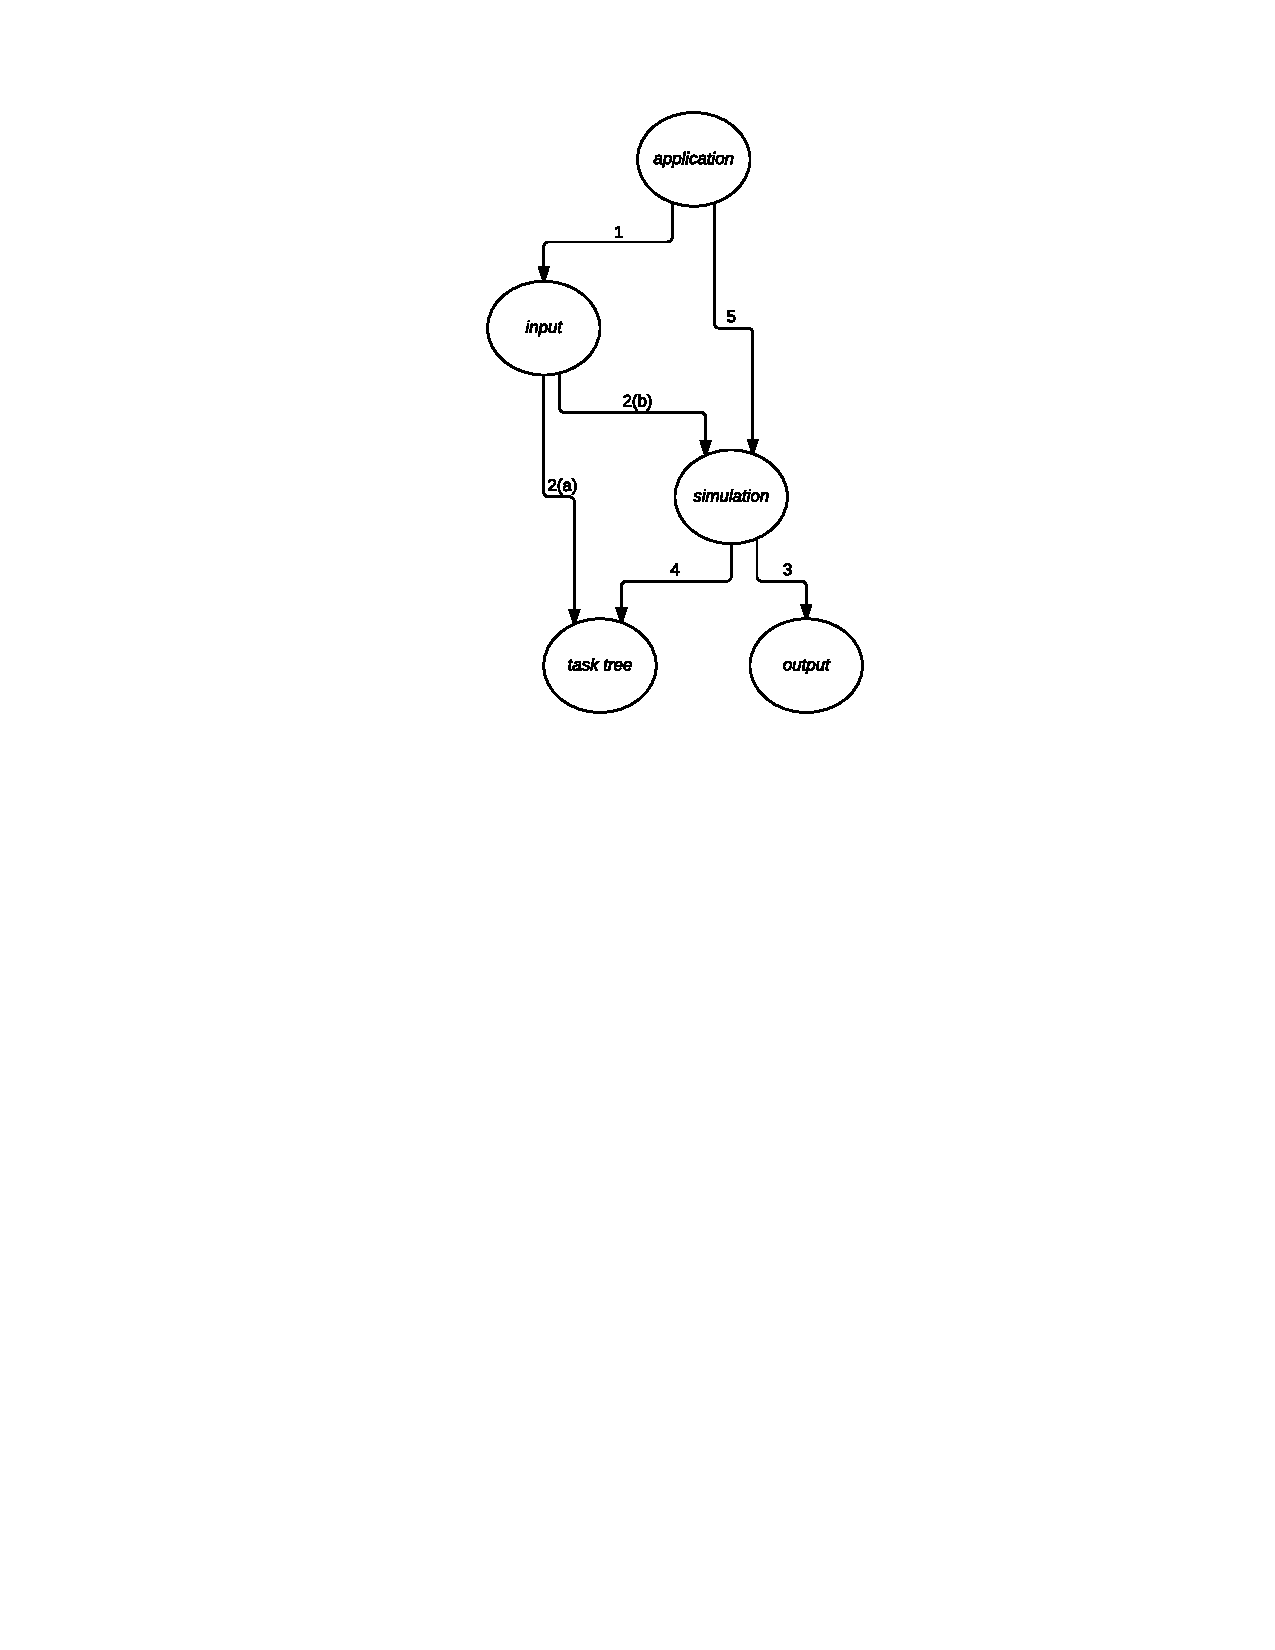
\includegraphics[trim=3.5cm 15.5cm 0cm 0cm, width=8.0in]{figs/OverviewUsesDiagram}
\caption{Overview of the USES diagram for packages within MASS.}
\label{fig:OverviewUsesDiagram }
\end{figure}

\textbf{Equivalence classes for Simulation File Input (SFI):} \\
Boundary Class: We don't support a boundary class in the Simulation File Input. We employ a strict format standard for the Simulation File Input. \\

Illegal Class: Wrongly Formatted Configuration File: We classify this scenario as an illegal class as this would result in the termination of the simulation. Any Simulation File Input (SFI) is considered to be wrongly formatted if it is unable to parse correctly. \\

Nominal Class: Correct Simulation File Input (SFI): We classify this scenario as a nominal class. Any correctly formatted Simulation File Input (SFI) would not cause a failure of the simulation. \\

\item \textbf{Output Module:} The output module takes in all the Agent communication transcriptions along with other statistical parameters and produce a Log File Output(LFO). \\

\textbf{Equivalence Classes for Log File Output(LFO):} \\

Boundary Class: We don't support a boundary class in the Log File Output. We employ a strict format standard for the Log File Output. \\

Illegal Class: In the event that an agent transcription does not reach the logger we classify this scenario as an illegal class. \\

Nominal Class: If all the transcriptions and statistics are recorded and filed by the Logger into the Log File Output we classify this scenario as a nominal class. \\

\item \textbf{Simulation Module:} The simulation module takes the parsed input files, and is responsible for the communication process with and between agents. Several unit tests have been performed on this module to insure its integrity. However we do intend to perform integration tests on the simulation package as well. \\

\end{itemize}

\item \textbf{System Testing:} After completing Integration tests we tested the system as a whole. We used several scenarios for the Simulation File Input and Configuration File Input files to rigorously check if the application meets all quality standards.

\item \textbf{User Acceptance Testing:} After completing all the Unit, Integration and System tests  we performed acceptance tests as per the clients requests to determine if the requirements of a specification are met. We were asked to incorporate some minor changes to the project which have been completed.

\end{itemize}

\end{enumerate}

\section{Testing Results}

\begin{enumerate}

\item \textbf{Sprint 3:} \\

After sprint 3 there are a total of  24  tests with 1 error, 0 skipped, 1 failures and a success rate of 91.6\%. The most significant packages are simulation, tasktree, input and output, however we had only performed tests on simulation, tasktree and output packages and had achieved instruction coverage of  51\%, 71\% and 64\%,  for the respective packages. The branch coverage for simulation package is 47\%, tasktree package is 76\%, and output package is 54\%.  We had achieved an overall instruction coverage of 47\% and a branch coverage of 42\%

\item \textbf{Sprint 4:} \\

After sprint 4 there are a total of 56 tests with 2 error, 0 skipped, 0 failures and a success rate of 96.43\%. The most significant packages are tasktree, input output, simulation with sub packages communication and simulatestate and have achieved instruction coverage of  100\%, 99\%, 93\%, 95\% and 97\%  for the respective packages. The branch coverage for communication subpackage in simulation package is 81\%, simulatestate subpackage in simulation package is 88\%, tasktree package is 93\%, input package is 89\% and output package is 92\%. The main application package is not tested in  sprint 4, but will be done before sprint 5. We have achieved an overall instruction coverage of 97\% and a branch coverage of 88\% .

\item \textbf{Sprint 5:} \\

After sprint 5 there are a total of 64 tests with 1 error, 0 skipped, 0 failures and a success rate of 98.44\%.The most significant packages are tasktree, input output, simulation with sub packages communication and simulatestate and have achieved instruction coverage of   99\%, 97\%, 92\%, 97\% and 99\% for the respective packages. The branch coveragefor communication subpackage in simulation package is 82\%,  simulatestate subpackage in simulation package is 85\%, tasktree package is 94\%, input package is 92\% and output package is 89\%. The thread creation and utilization does tend to vary the coverage but is not significant an alternate way to get a higher coverage is to create integration tests for the modules using threads. We have achieved an overall instruction coverage of 97\% and a branch coverage of 88\% .

\item \textbf{Sprint 6:} \\

After sprint 6 there are a total of 75 tests with 0 errors, 0 skipped, 0 failure and a success rate was 100\%. We have achieved instruction coverage of 93\%, 94\%, 99\%, 98\% and 100\% for input, output, tasktree, simulatestate subpackage in simulation and communication subpackage in simulation packages respectively. The Branch coverage for input, output, tasktree, simulatestate and communication packages are 91\%, 91\%, 79\%, 87\% and 84\% respectively. The thread creation and utilization does tend to vary the coverage in the communication package but is insignificant. After completing sprint 6 we have achieved an overall instruction coverage of 98\% and a branch coverage of 87\%.


\end{enumerate}